\section{Aufbau und Durchführung} % (fold)
\label{sec:aufbau_und_durchf_hrung}


	\subsection{He-Kanne und Füllstandmessung} % (fold)
	\label{sub:f_llstandmessung}
	
		Der prinzipielle Aufbau der He-Kanne ist in Abbildung \ref{hecan} zu sehen. 
		Der isolierte und abgeschirmte Heliumbehälter befindet sich unterhalb einer zusätzlichen Stickstoffkühlung, die die unmittelbare Umgebung des He auf ca. $80 \unit{K}$ abkühlt bevor der äußere Mantel der Kanne kommt.
		\begin{figure}[H]
			\center
			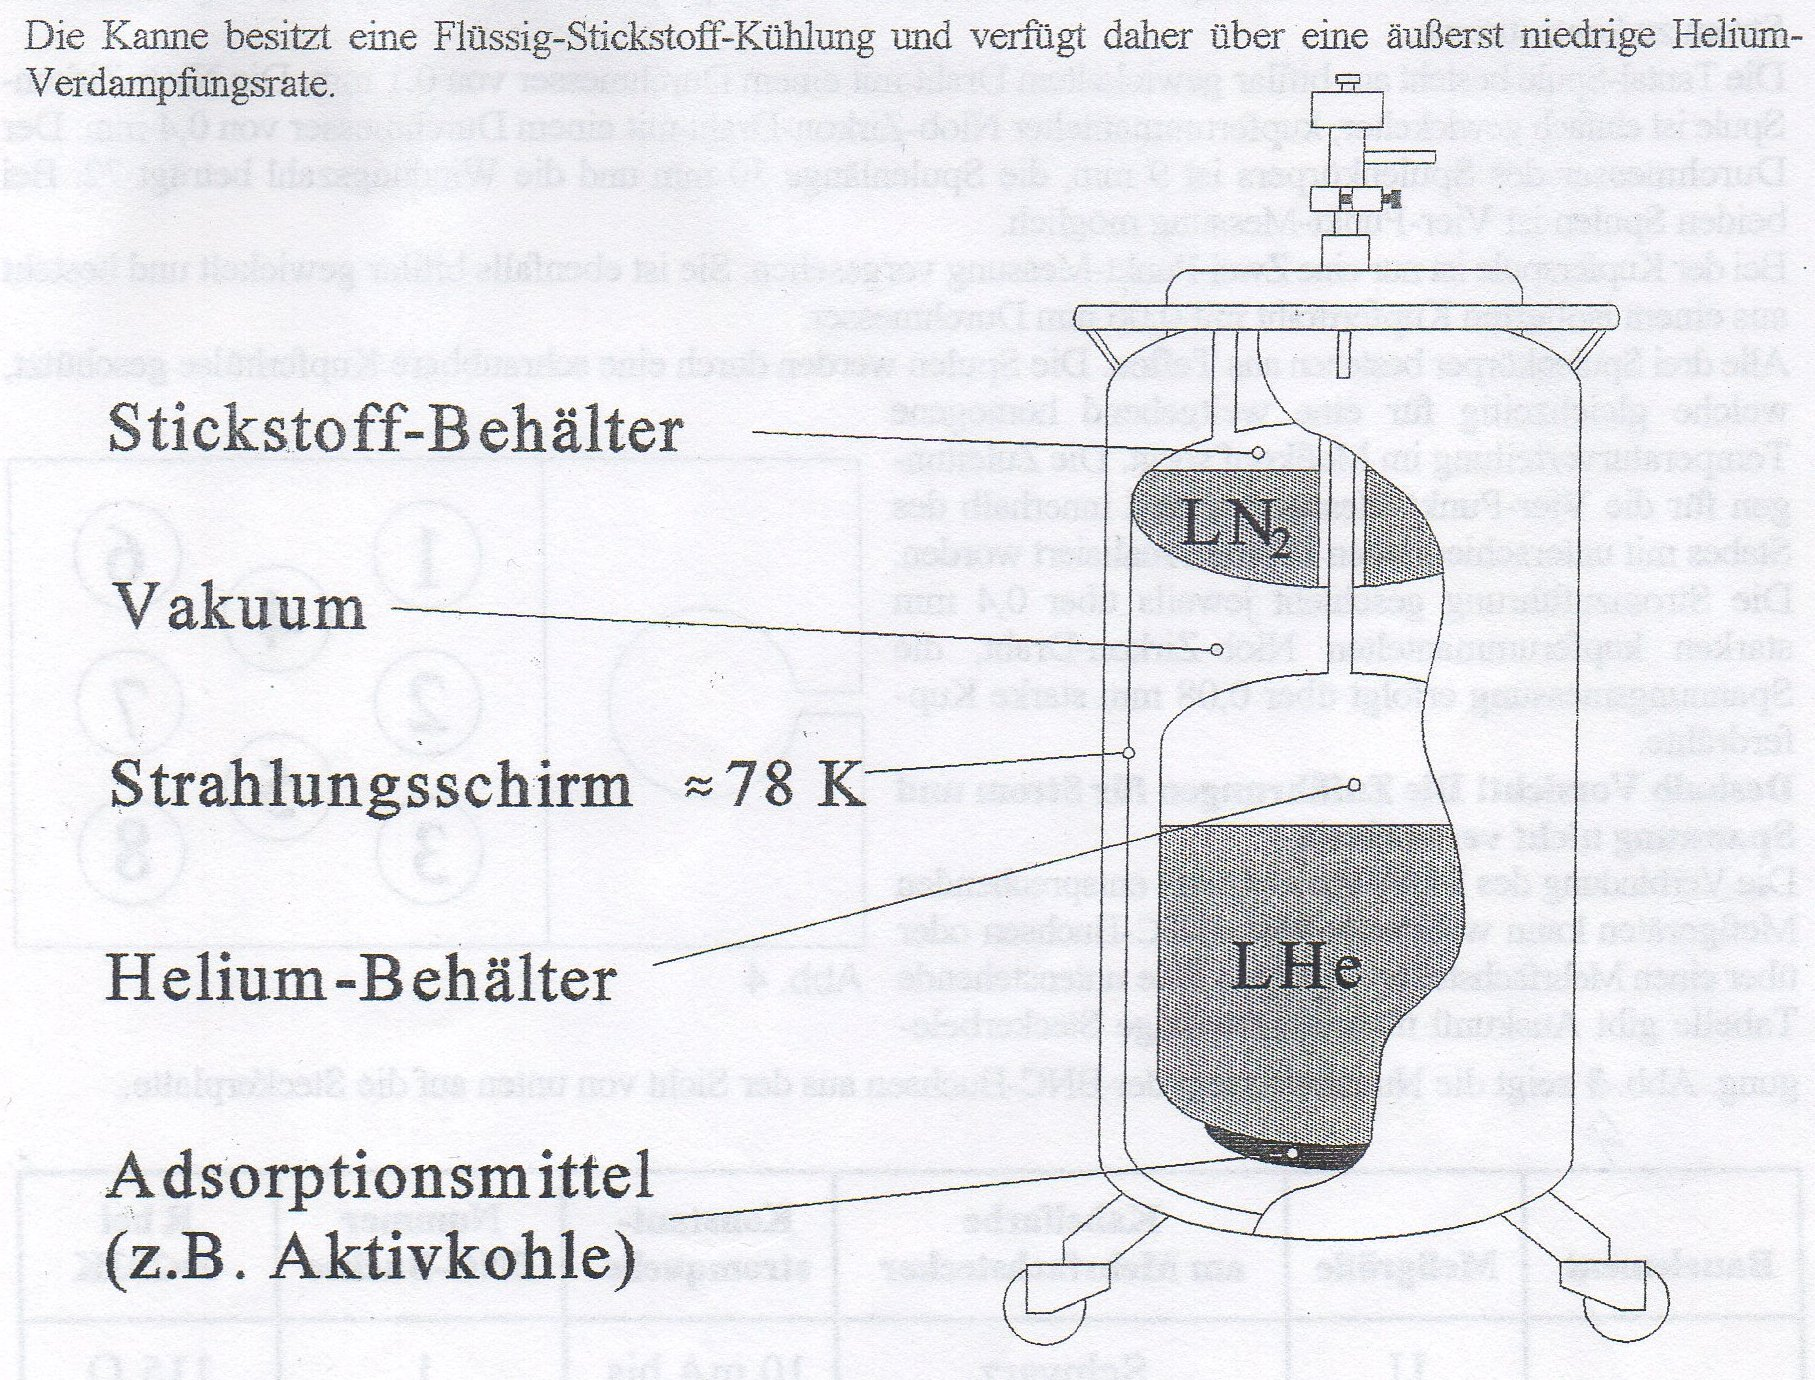
\includegraphics[scale=0.7]{messwerte/hecan.jpg}
			\caption{Aufbau der verwendeten Helium-Kanne (nach Versuchsunterlagen)}
			\label{hecan}
		\end{figure}
		Zur Füllstandsmessung des flüssigen Stickstoffs wird ein kleiner Kunststoffstab in das Reservoir getaucht und nach kurzer Zeit wieder zügig entfernt. 
		Die am kalten Stab ausfrierende Luftfeuchtigkeit zeigt dann den $N_2$ an.
		Um die Pegelhöhe des He abzuschätzen wird ein dünnes Metallrohr, das mit einer Gummimembran abgeschlossen ist in der Kanne versenkt.
		Ein Gummipfropfen am Rohr schließt dabei die Kanne luftdicht ab.
		Im Rohr entstehen nun durch die unterschiedlichen Druck und Temperaturverhältnisse thermoakustische Schwingungen, deren Frequenz schlagartig und hörbar tiefer wird, sobald der Stab die Oberfläche des flüssigen Heliums erreicht.

	% subsection f_llstandmessung (end)


	\subsection{Aufbau des Messstabes} % (fold)
	\label{sub:aufbau_des_messstabes}

		Alle Geräte und Materialien, die direkt mit dem flüssigen He in Kontakt kommen sollen, befinden sich am Ende des Messstabes.
		Dieser besteht neben dem Messkopf und Zuleitungsrohr aus einer aufschraubbaren Niob-Hülse, die bei tiefen Temperaturen ebenfalls supraleitet und äußere Magnetfelder abschirmt.
		Im Messkopf befinden sich Pt1000-Widerstand, Diode, bifilare Kupfer- und Tantal-Spule sowie eine einfach gewickelte Niob-Zirkon-Spule zur Erzeugung definierter Magnetfelder.
		Alle Elemente sind über BNC-Buchsen am oberen Stabende anzusteuern.
		Die erforderliche Vierdrahtmessung ist so bereits im Stab integriert.
		Der Aufbau des Messkopfes ist in Abbildung \ref{head} zu sehen:
		\begin{figure}[H]
			\center
			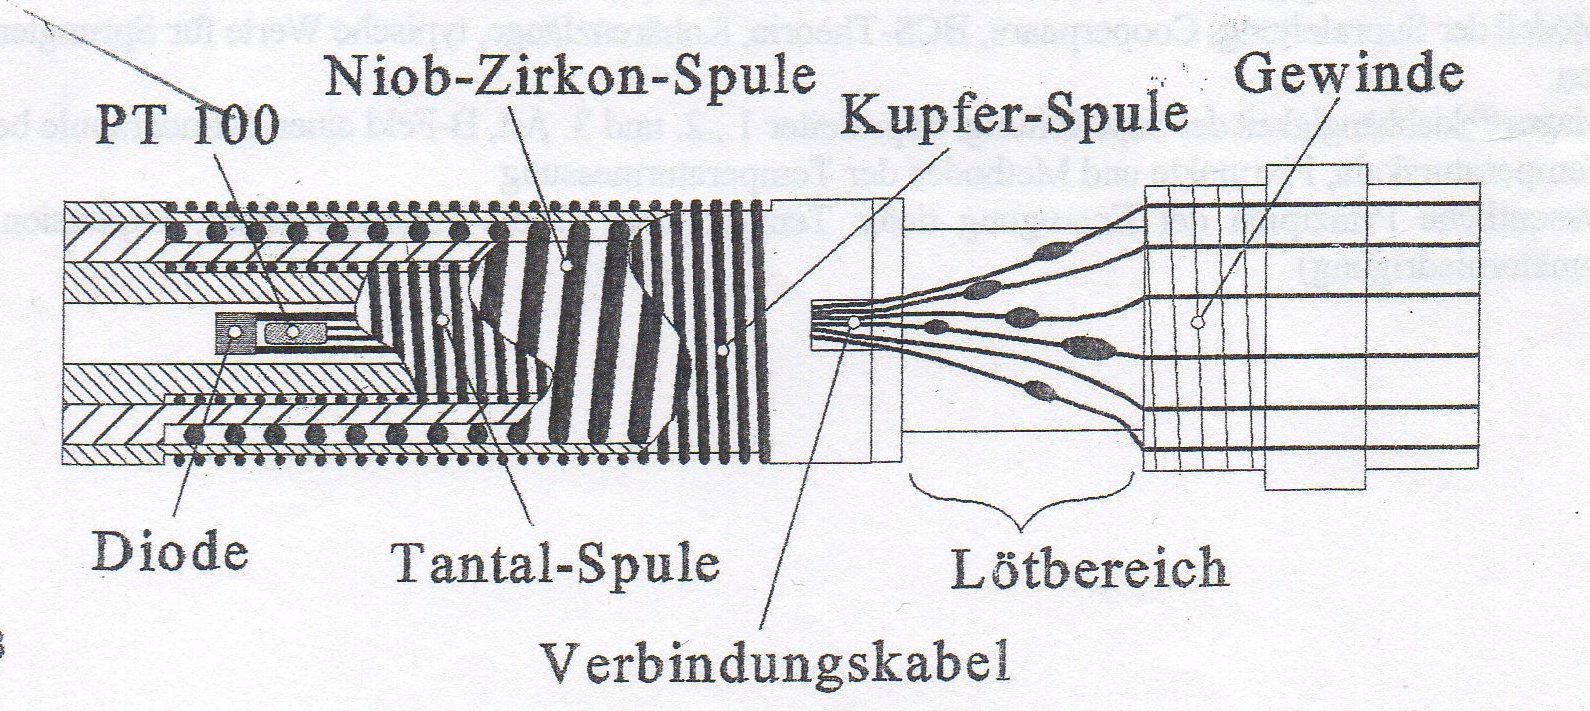
\includegraphics[scale=0.7]{messwerte/head.jpg}
			\caption{Aufbau des verwendeten Messkopfes (nach den Versuchsunterlagen)}
			\label{head}
		\end{figure}
	
	% subsection aufbau_des_messstabes (end)


	\subsection{Stromversorgung, Versuchsplatz und Aufzeichnung} % (fold)
	\label{sub:stromversorgung_versuchsplatz_und_aufzeichnung}
	
		Die Elemente werden über eine Konstantstromquelle versorgt.
		Verwendet wurde hierzu die Vierfachumpolkonstantstromquellenfortgeschrittenenpraktikumsgeräteeinheit.
		Um Störungen durch den Netzwechselstrom zu vermeiden sind die meisten Geräte batteriebetrieben.
		Zusätzliche Vor- und Parallelwiderstände können (über eine vietnamesische Weichblechdose) zugeschaltet werden um während der Montage die Geräte vor unbeabsichtigten Spannungs- oder Stromspitzen zu schützen.
		Die Aufzeichnung der Messwerte kann über einen Analog-Digital-Wandler und einen LabView-XY-Schreiber erfolgen.
		Ein Foto vom Versuchsplatz ist in Abbildung \ref{platz} beigefügt.
		\begin{figure}[H]
			\center
			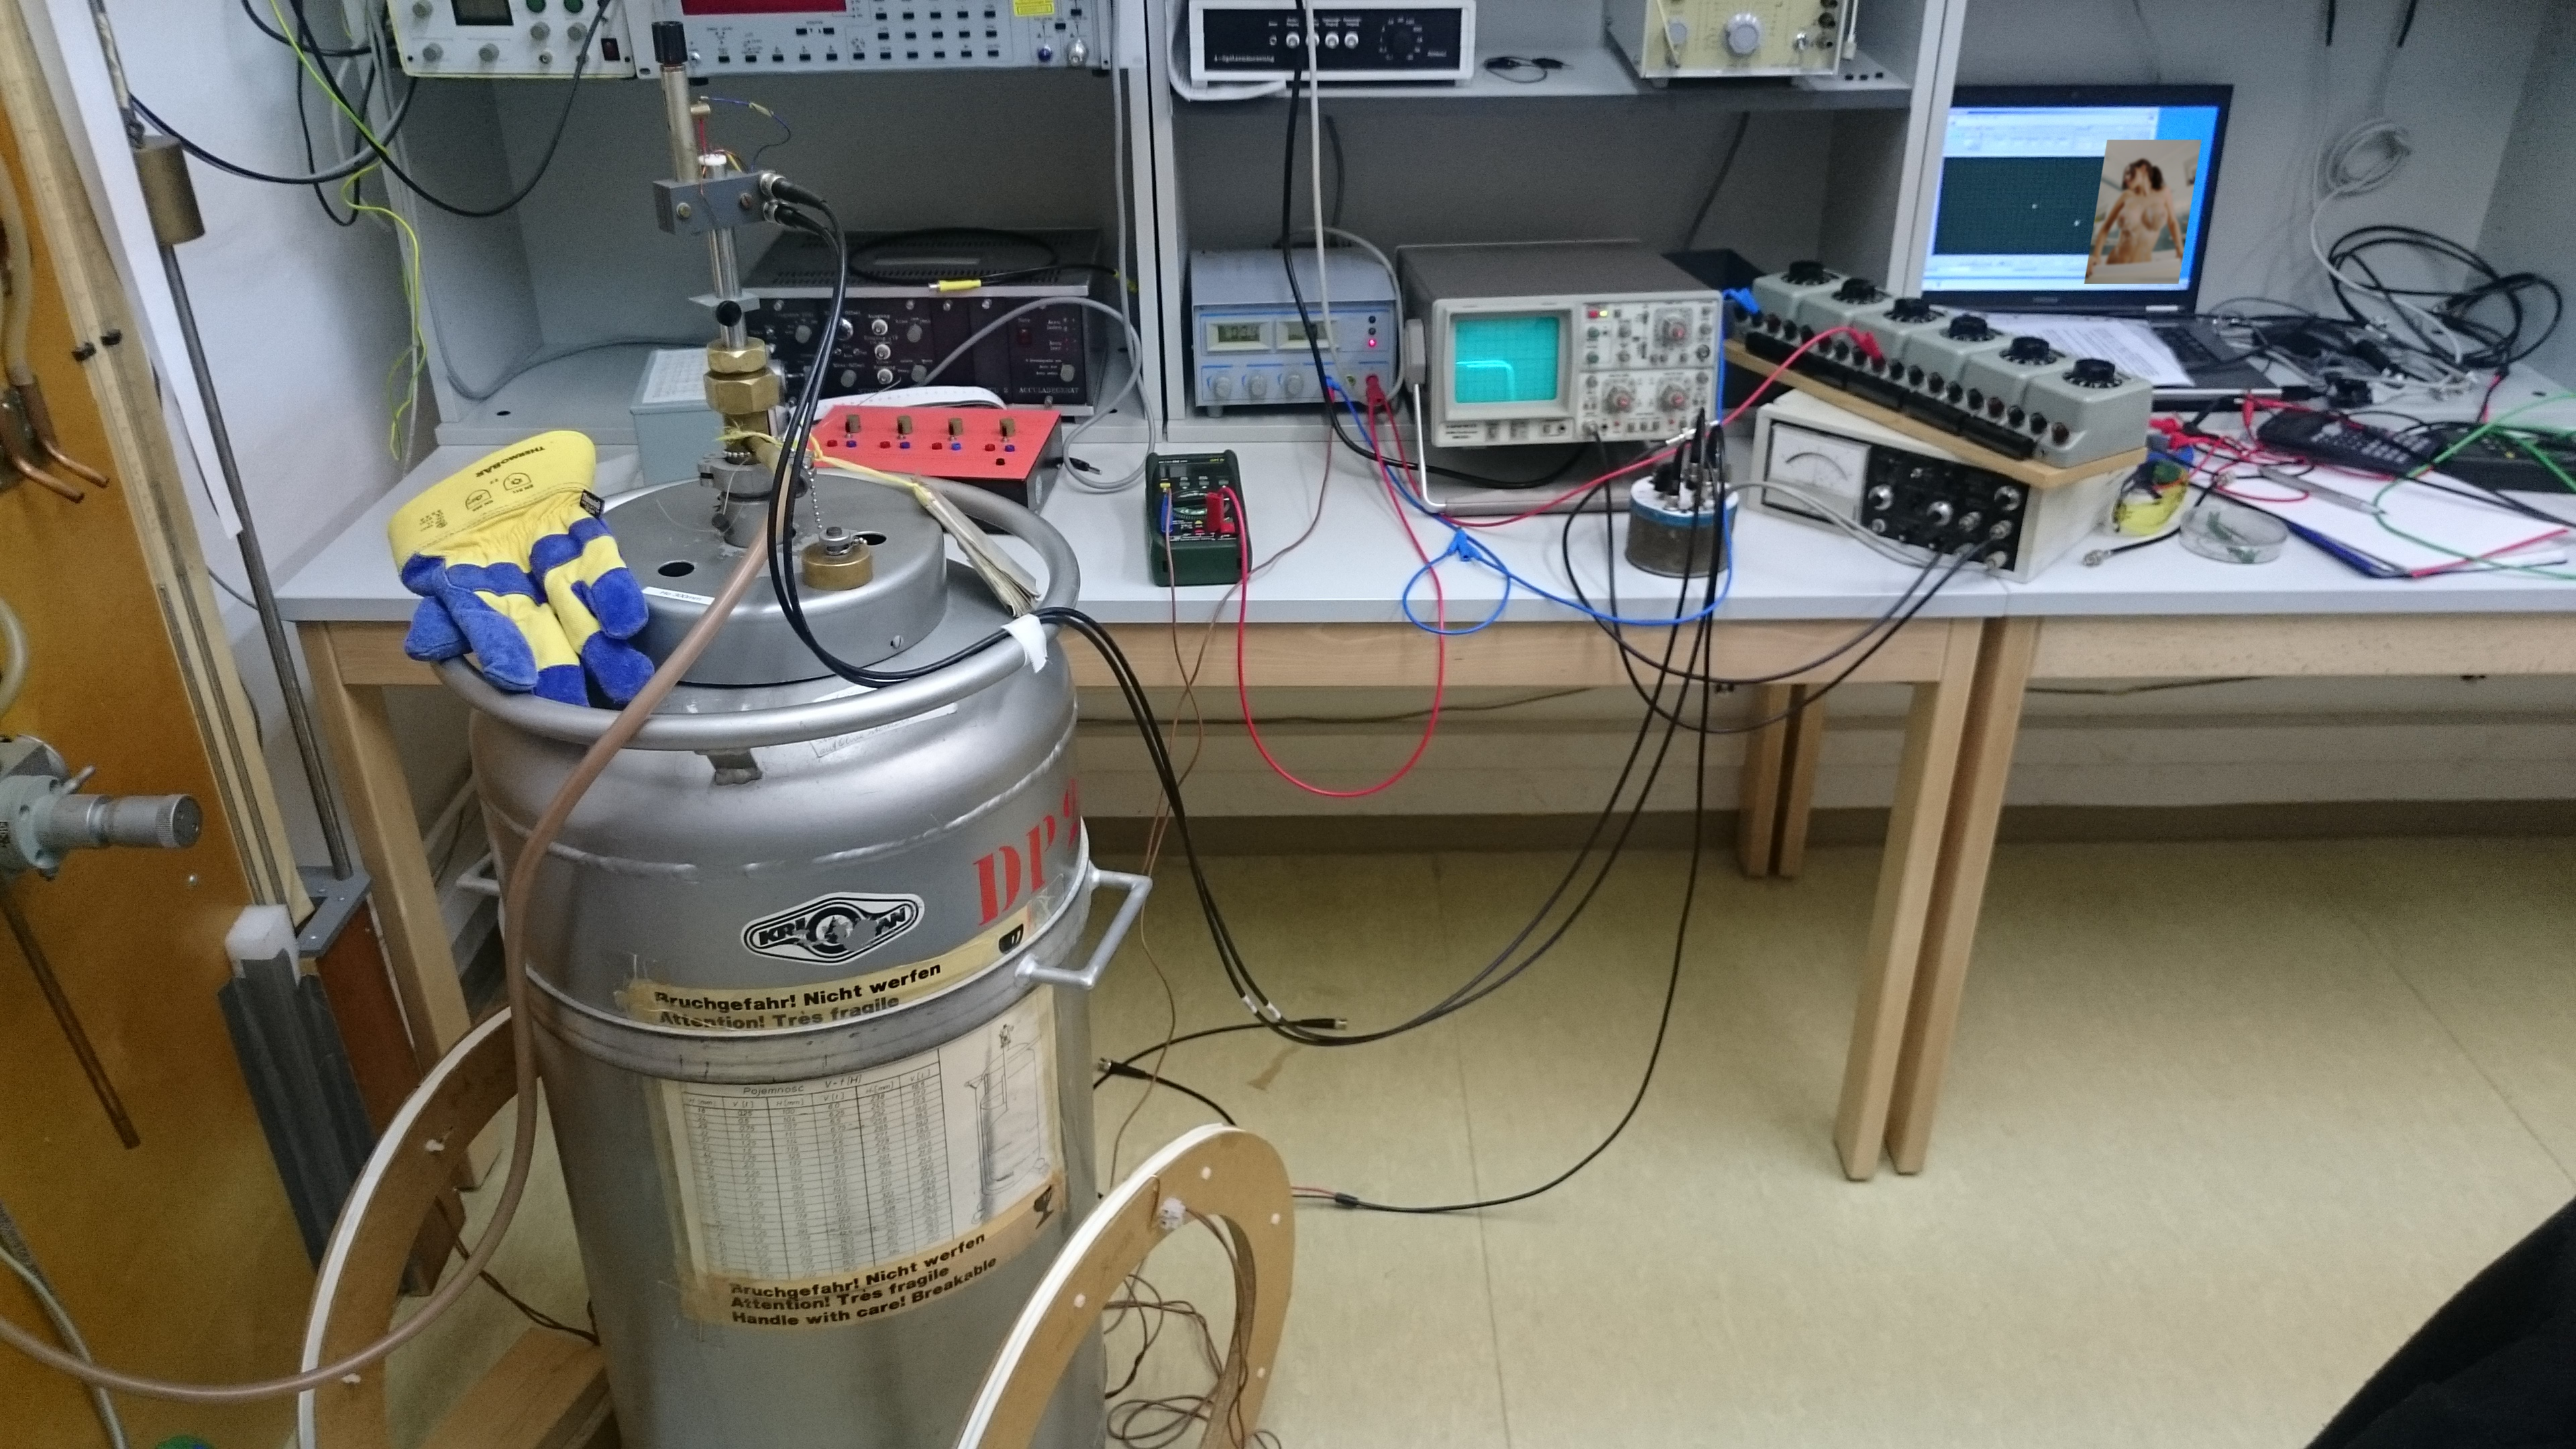
\includegraphics[scale=0.08]{messwerte/DSC_0631_booble_blazer_2.JPG}
			\caption{Versuchsplatz mit fast allen verwendeten Geräten}
			 % außer dem Kaffeeautomaten und anderen diversen allerdings eigentlich nützlichen Geräten, die wir eigentlich hätten verwenden SOLLEN}
			\label{platz}
		\end{figure}

	% subsection stromversorgung_versuchsplatz_und_aufzeichnung (end)


	\subsection{Josephson-Kontakte} % (fold)
	\label{sub:josephson_kontakte}

		Die Josephson-Kontakte befinden ebenfalls am Ende des Messstabes.
		Beim Gleichstrom-Josephson-Effekt werden über einen Bautenzug zwei Niob-Drahtspitzen an einander gedrückt.
		Da sich auf ihrer Oberfläche wie bei den meisten Metallen eine Oxidschicht befindet, ist die isolierende Barriereschicht bereits vorhanden.
		Durch leichte Bewegung des Bautenzugs kann mit etwas Geschick der gewünschte Kontakt erzeugt werden.
		Die Einkopplung der Mikrowellen des 8mm-Klystrons erfolgt am oberen Ende des Stabes.
		\\
		Der für die Magnetfeldmessung benötigte SQUID-Ring wird mit Hilfe der Methode der gekreuzten Drähte erzeugt.
		Naja, zumindest haben wir es auf diese Weise versucht.
		Dabei werden 2 gekreuzte, mit Oxidschicht überzogene Niob-Drähte wieder mittels eines Bautenzugs in leichten Kontakt gebracht.
		Mit etwas Glück und Geschick (in etwa so viel, dass man 3 rohe Eier senkrecht übereinander stapeln könnte) berühren sich die Drähte dann nur in zwei Punkten, die die beiden SIS (Supraleiter-Isolator-Supraleiter) Kontakte darstellen.
		Falls mehrere Kontaktstellen auftreten (und das tun sie), sind die auftretenden Stromminima weniger tief.
		Das angelegte Magnetfeld wurde mit Hilfe zweier Helmhotzspulen erzeugt und über eine Konstantstromversorgung mit eingeschalteter Dekadenreihe als Stromteiler konnten Strom- und Feldstärke sehr genau eingestellt werden.

	
	% subsection josephson_kontakte (end)

% section aufbau_und_durchf_hrung (end)